\documentclass{article}
\usepackage{tikz}
\usepackage{dsfont}
\usetikzlibrary{matrix}
\newcommand*\Z{\mathds{Z}}
\newcommand*\ZZ{|[draw,circle]| \Z_2}
\begin{document}
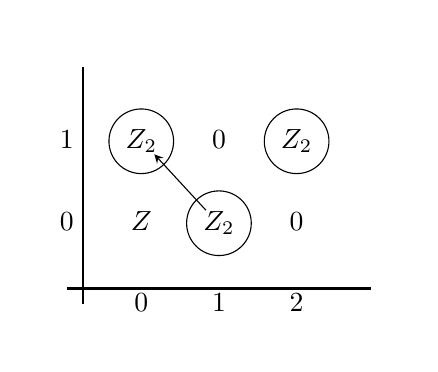
\begin{tikzpicture}
  \matrix (m) [matrix of math nodes,
    nodes in empty cells,nodes={minimum width=5ex,
    minimum height=5ex,outer sep=-5pt},
    column sep=1ex,row sep=1ex]{
                &      &     &     & \\
          1     &  \ZZ &  0  & \ZZ & \\
          0     &  \Z  & \ZZ &  0  & \\
    \quad\strut &   0  &  1  &  2  & \strut \\};
  \draw[-stealth] (m-3-3.north west) -- (m-2-2.south east);
\draw[thick] (m-1-1.east) -- (m-4-1.east) ;
\draw[thick] (m-4-1.north) -- (m-4-5.north) ;
\end{tikzpicture}
\end{document}